
%%%%%%%%%%%%%%%%%%%%%%%%%%%%%%%%%%%%%%%%%%%%%%%%%%%%%%%%%%%%%%%%%%%%%%%%%%%%%%%%
%% CAPITULO
%%%%%%%%%%%%%%%%%%%%%%%%%%%%%%%%%%%%%%%%%%%%%%%%%%%%%%%%%%%%%%%%%%%%%%%%%%%%%%%%
\chapterimage{chapter_head_2.pdf} % Chapter heading image

\chapter{\textcolor{blue}{Historia do samba de gafieira}}
\index{Historia do samba de gafieira}


O samba de gafieira, como dança, descende principalmente do maxixe (dança),
que a sua vez foi gerado  pela união do  lundu, 
a polca e outras danças europeias.
Assim, misturando o maxixe com a ginga, e o ritmo de outras danças africanas, 
é que se obteve o que agora chamaríamos como o samba de gafieira (primigênio)\footnote{
Primitivo; primordial; o primeiro da sua espécie. = PRIMÍGENO \cite{priberamprimigenio}.
} \cite[pp. 139]{perna2002samba}.
\begin{definition}[Maxixe:]
\index{Dança!Maxixe}
Esta é uma dança urbana afro-brasileira \cite[pp. 4]{musicasambavariasdef1}, 
em compasso binário, surgida em Rio de Janeiro, 
na Cidade Nova e nos cabarés de Lapa \cite[pp. 465]{marcondes1977enciclopedia}  \cite[pp. 198]{dourado2004dicionario}, 
aproximadamente entre 1870 e 1880 \cite[pp. 465]{marcondes1977enciclopedia}  \cite[pp. 62]{reinato2010musica}.

A dança era considerada de baixe ralé pela sociedade local, 
pois era entendida como um modismo indecente das classes baixas, imoral como o Lundu \cite[pp. 198]{dourado2004dicionario}.
Esta dança recebeu influencias da polca \cite[pp. 198]{dourado2004dicionario} e da Habanera \cite[pp. 62]{reinato2010musica}.

O maxixe tinha uma boa quantidade de passos como: 
parafuso, 
janela,
jocotó
saca-rolha, 
balão, 
balão apagado,
balão caindo,
corta-jaca,
urubu malandro,
sino, 
carrapeta, 
corta-capim, 
\cite[pp. 465]{marcondes1977enciclopedia} \cite[pp. 68, 129, 131,173]{efege1974maxixe} etc. 
Num principio o maxixe era dançado nas músicas de tango, havanera, polca e lundu; 
e só foi ate o final do século XIX que ganhou uma música com gênero próprio \cite[pp. 465]{marcondes1977enciclopedia}.

No inícios do século XX o maxixe foi exportado e dançado na Europa, atingindo um grande sucesso, 
chegando a ser apresentado pelo dançarino ``Duque'' em Paris (1914) e em Londres (1922) \cite[pp. 465]{marcondes1977enciclopedia}.
Este dançarino é considerado o civilizador do maxixe \cite[pp. 129]{efege1974maxixe}.

Uma explicação muito interessante do maxixe é cantada pela atriz, Aurélia Delorme,
numa representação num quadro de revista, interpretando  ``Maxixe Aristocrático'' (1904, José Nunes), 
que arrancava aplausos e provocava pedidos de bis;
o seguinte texto indica sua pauta \cite[pp. 80-81]{efege1974maxixe} \cite{REIS2003}: 
\begin{citando}
O maxixe tem ciência,\\
ou pelo menos tem arte.\\
Para haver proficiência\\
basta mexer certa parte.\\
Pois o próprio Padre Santo,\\
sabendo o gosto que tem,\\
virá de Roma ao Brasil\\
dançar maxixe também.\\ 
\end{citando}
\end{definition}
\begin{definition}[Lundu:] 
\index{Dança!Lundu}
Esta é uma dança, brasileira, de roda e umbigada; esta teve sua origem no batuque dos bantos africanos,
e provavelmente trazida de Angola pelos escravos na segunda metade do século XVIII \cite[pp. 198]{dourado2004dicionario}.
Posteriormente foi introduzida aos salões das cortes do Brasil e Portugal.
No Brasil esta dança teve influencias da ``Modinha''(Portuguesa) e do ``Fandango''(Espanhol) \cite[pp. 198]{dourado2004dicionario}.
\end{definition}


A Figura \ref{fig:formuladosambagafieira} mostra a árvore genealógico do samba de gafieira (primigênio),
visto quando o samba fez sua aparição nos salões de dança denominados gafieiras.
\begin{figure}[h]
  \centering
  \begin{subfigure}[b]{0.535\textwidth}
    \centering
    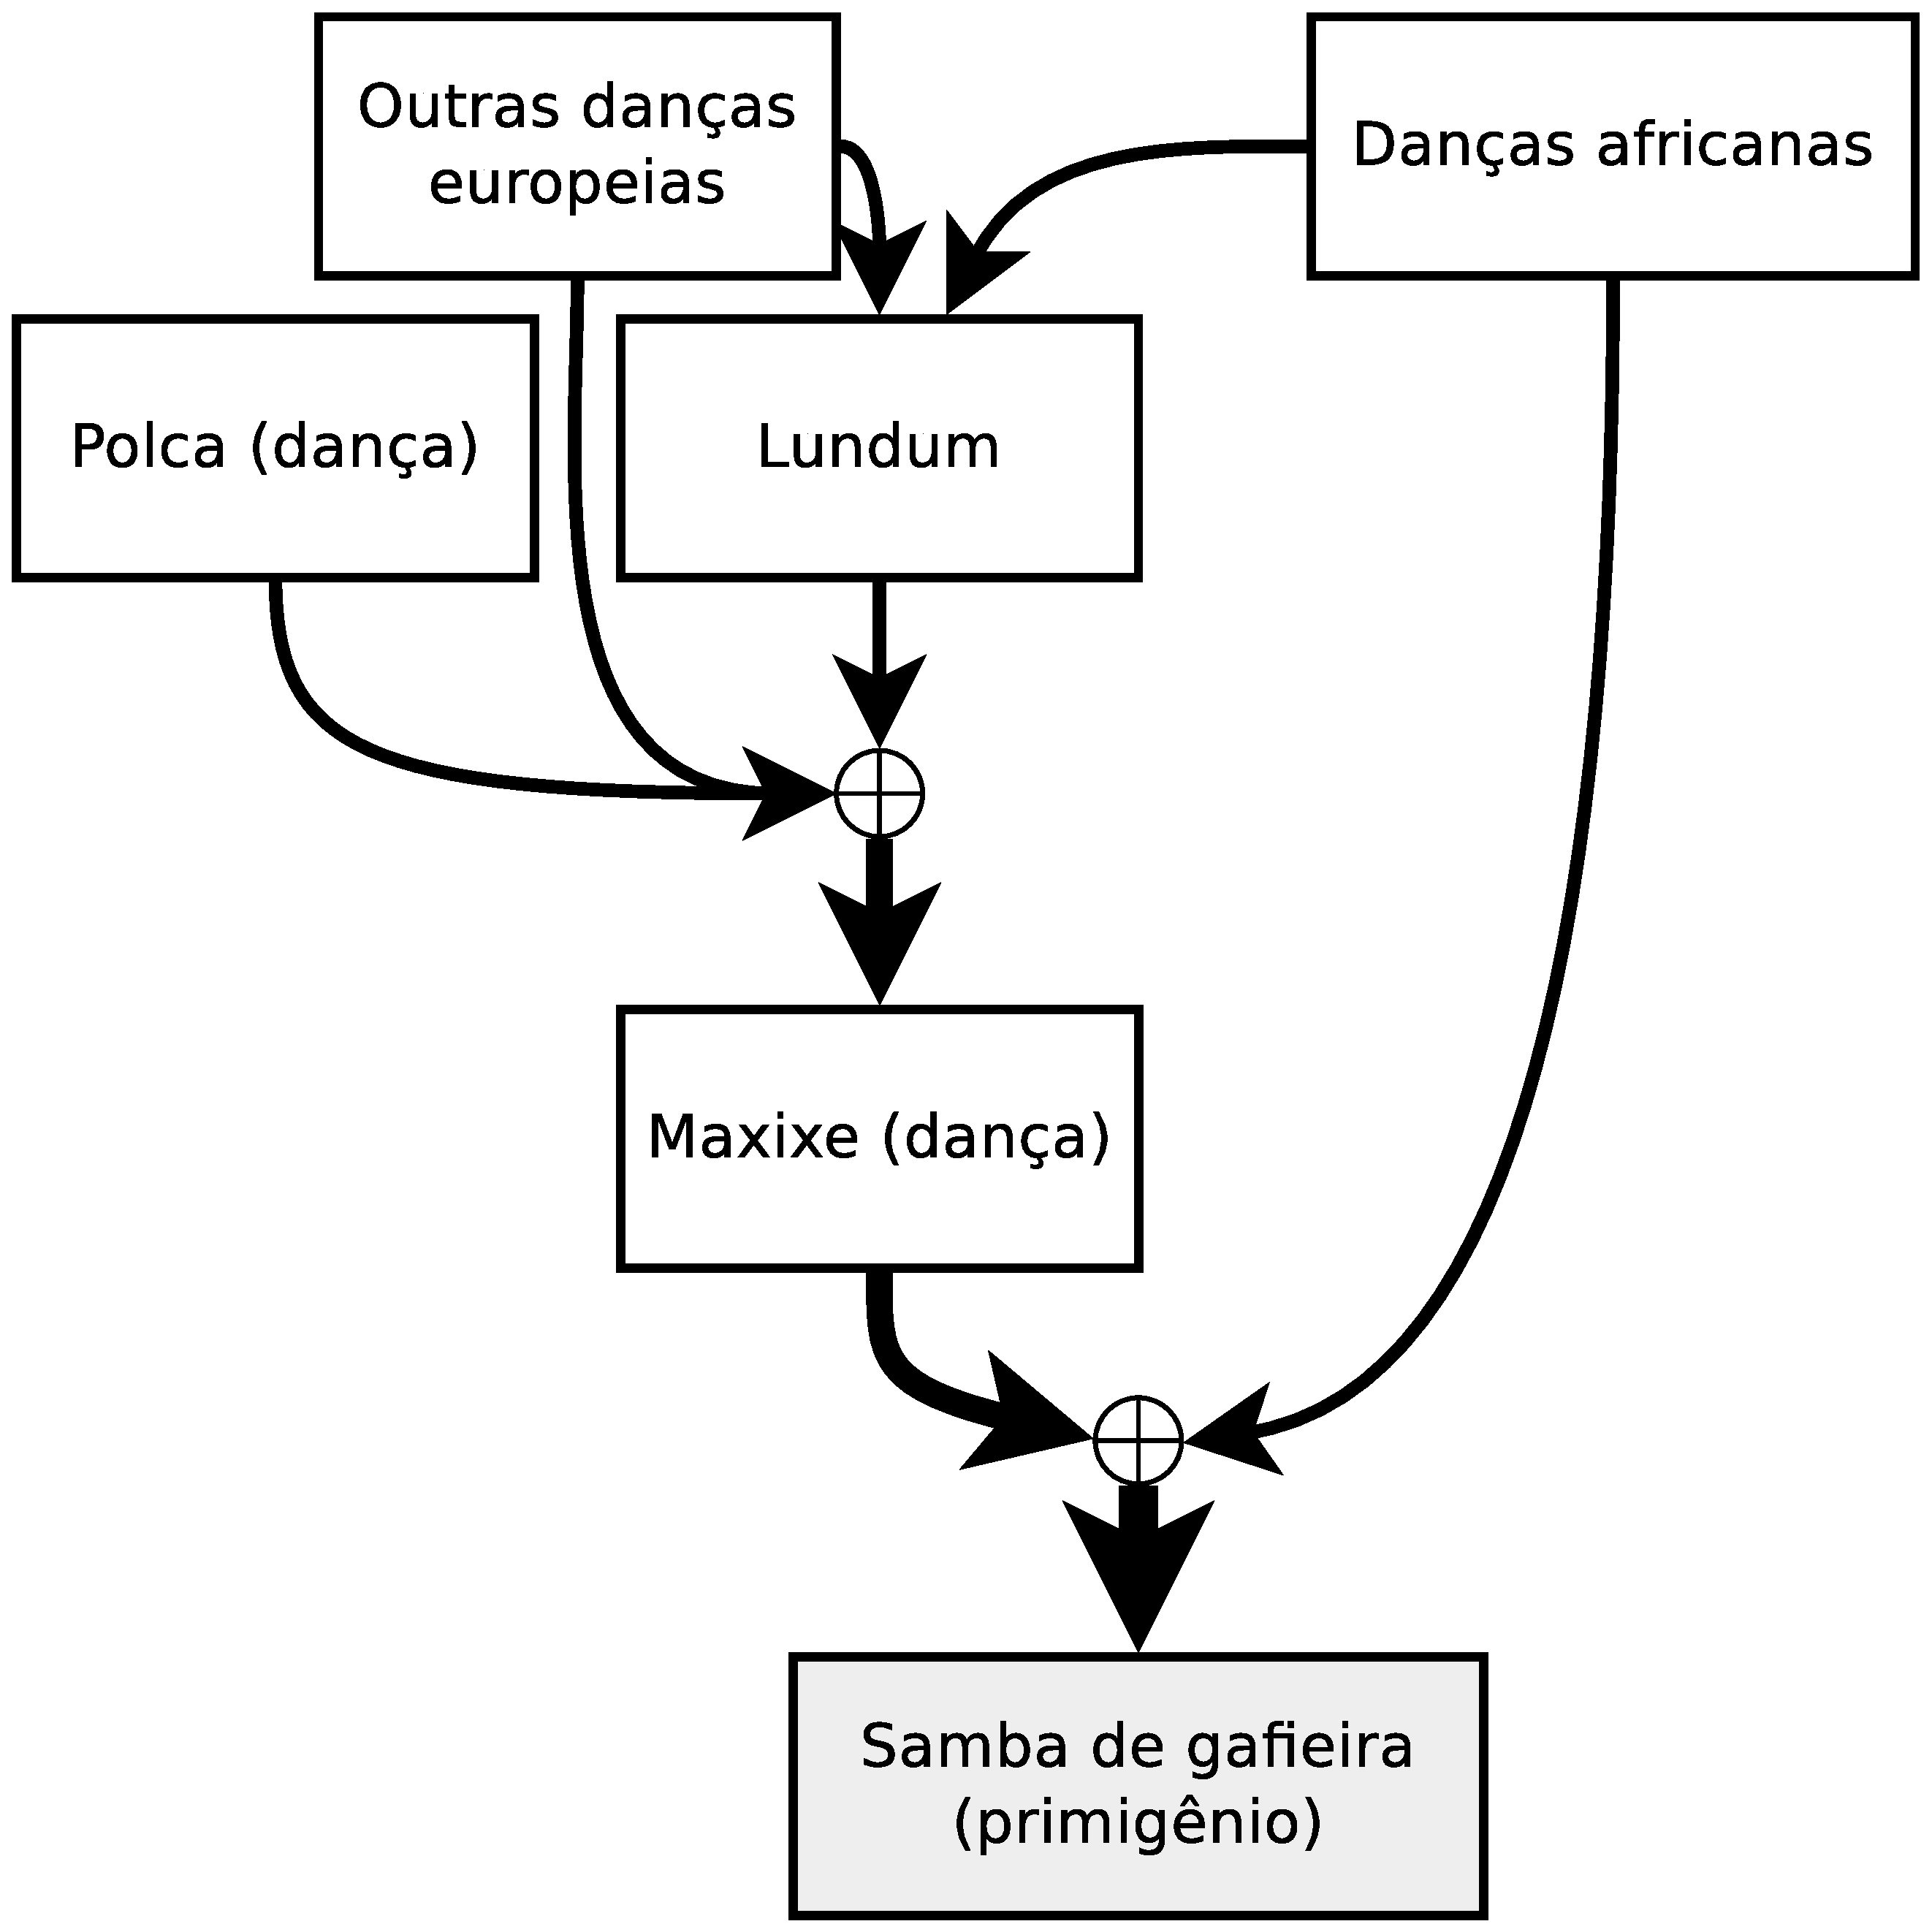
\includegraphics[width=\textwidth]{chapters/cap-historia-sambagafieira/sambagafieiraformula.eps}
    \caption{Formação do samba de gafieira (primigênio).}
    \label{fig:formuladosambagafieira}
  \end{subfigure}
  \begin{subfigure}[b]{0.385\textwidth}
    \centering
    \includegraphics[width=\textwidth]{chapters/cap-historia-sambagafieira/sambagafieiraformula2.eps}
    \caption{Formação do samba de gafieira (atual).}
    \label{fig:formuladosambagafieira2}
  \end{subfigure}
\caption{Formula da criação do samba de gafieira.}
\label{fig:formuladosambagafieiraall}
\end{figure}


O aparecimento do samba nos salões de dança, 
foi um grande impacto para as pessoas que frequentavam estes lugares;
sendo considerado um ritmo novo e ligeiro,
que desagradou aos bailarinos de maior idade e menos ágeis \cite[pp. 6 - cad. B]{entrevistajuliojournalbrasil1}.
O senhor, Júlio Simões, socio da ``Kananga do Japão'' e
do ``Elite Club'', chegou a temer pelo futuro do seus empreendimentos; porem, para sorte dele, 
o samba fez muito sucesso no Elite,
e passou a ser considerado vestibular indispensável para qualquer pessoa que pretendesse ser bailarino, 
compositor ou instrumentista \cite[pp. 6 - cad. B]{entrevistajuliojournalbrasil1}.

Pode-se estabelecer o ingresso do samba, aos salões de dança, entre os anos de 1930 e 1940 \cite[pp. 140]{perna2002samba}.
Para o ano de 1940 o samba dançado em salões, já tinha ganhado muita força;
porem, podia-se ver 3 formas diferentes de ser dançado \cite[pp. 142-143]{perna2002samba}:
\begin{itemize}
\item \textbf{Samba-canção (dança)},
\index{Dança!Samba-canção} 
que agora é um modo de dança extinto \cite[pp. 143]{perna2002samba}.

\item \textbf{Samba-batucada},
\index{Dança!Samba-batucada} 
que é o samba de gafieira (primigênio) \cite[pp. 143]{perna2002samba}.
Existe uma menção sobre este estilo no ``Jornal do Brasil'', no dia 9 de janeiro de 1938,
onde se indica \cite[pp. 4]{musicasambavariasdef1}:
\begin{citando}%%
Tentativas isoladas de puro 
snobismo e ás vezes de compreensão 
inexata da origem da 
musica e dansa, chamam-no de samba jongo, \textbf{samba batucada} ou
pretendem mistura-lo com o fox, -- samba fox ou com sumba samba rumba.
\end{citando}
\item \textbf{Samba liso}, 
\index{Dança!Samba liso}
que é um estilo de dança que perdura ainda ate nossos dias \cite[pp. 143]{perna2002samba}, ver Seção \ref{subsec:estilosdedanca}.
\end{itemize}

Com o passar dos anos foram agregados elementos de outras danças a esse primitivo, samba de gafieira;
por exemplo, movimentos do tango e do rock \cite[pp. 142]{perna2002samba}, 
obtendo assim a forma de dança que vemos hoje em dia, ver Figura \ref{fig:formuladosambagafieira2}.

Asim, podemos falar do samba de gafieira como dança, só apos da aparição do samba nos
salões de dança abertos ao público, e a partir da criação do termo gafieira pra definir a estes lugares.
Com a mistura destes dois acontecimentos obtemos o termo, samba de gafieira,
que iniciou seu caminho na dança, mas como uma descrição do âmbito da dança (e da música), que como nome próprio.
Porem, a formação dos movimentos e corporalidade desta dança tem um caminho que data desde muito tempo atrás.
A Figura \ref{fig:sambagafieiracrono} mostra a cronologia do uso do termo samba de gafieira. 

\begin{figure}[h]
  \centering
    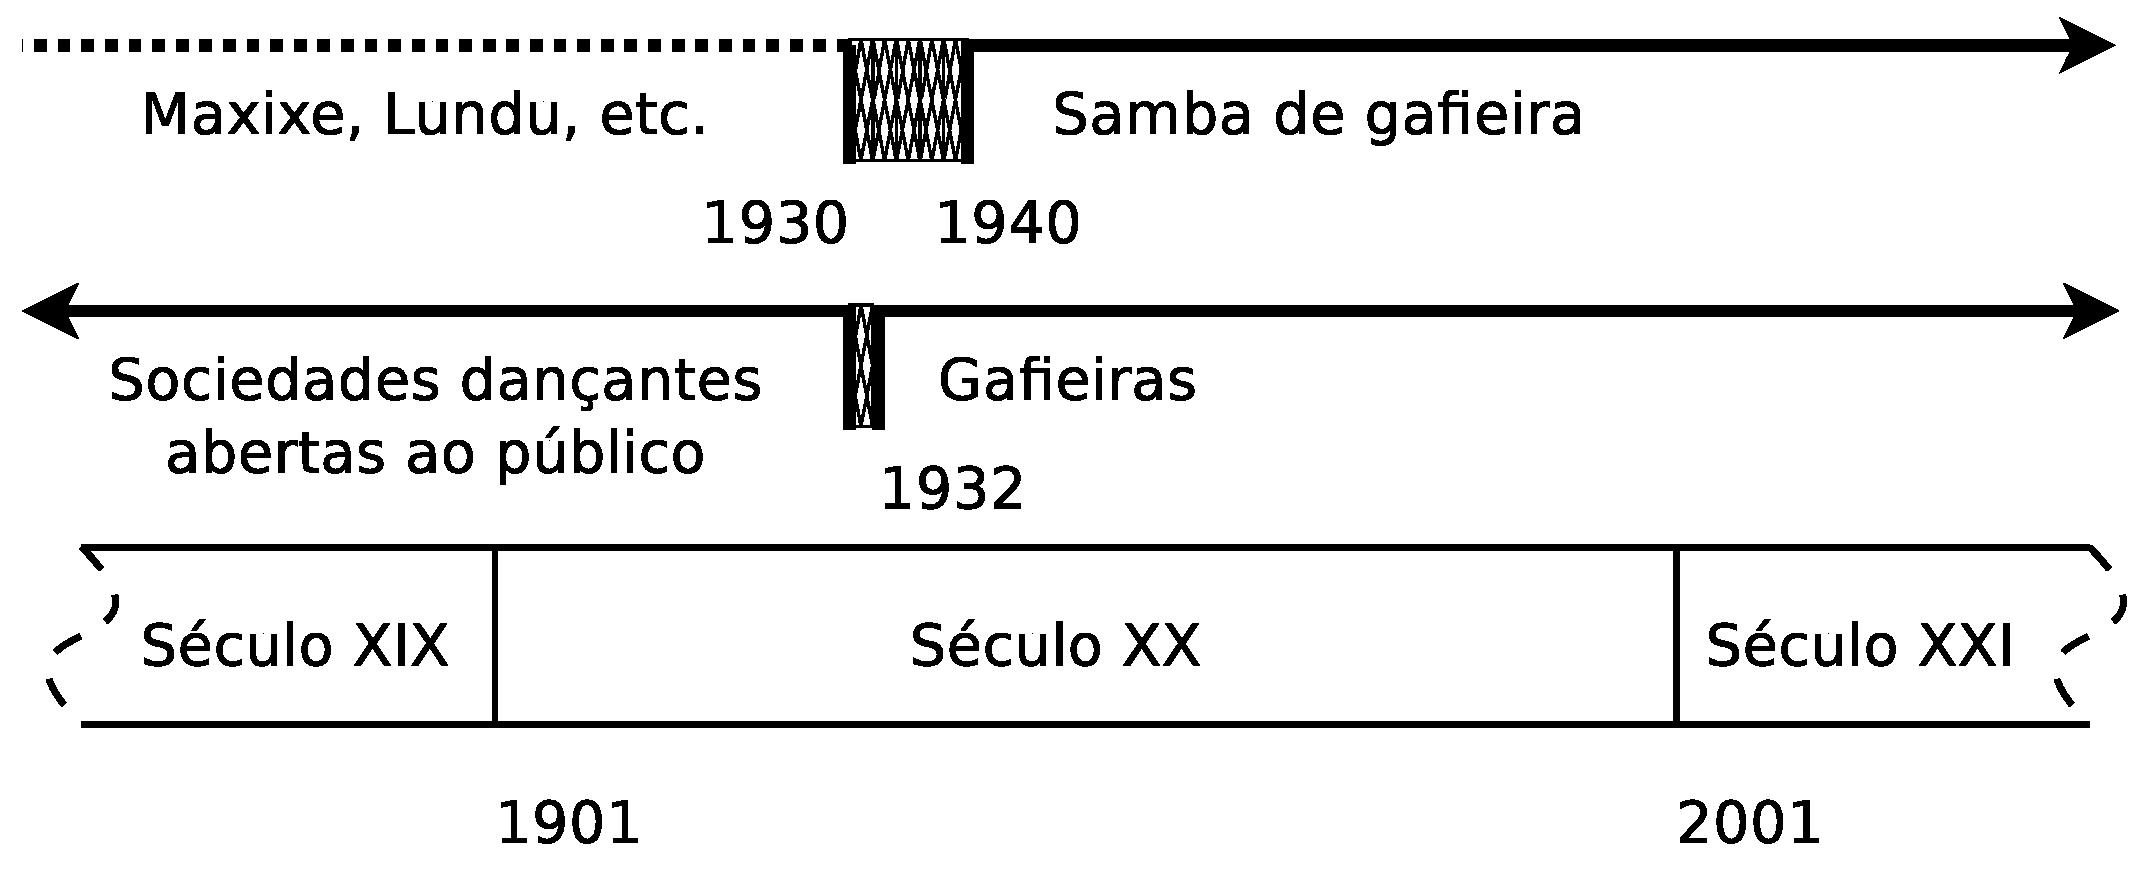
\includegraphics[width=0.7\textwidth]{chapters/cap-historia-sambagafieira/gafieira-crono.eps}
  \caption{ Cronologia da formação do samba de gafieira.}
\label{fig:sambagafieiracrono}
\end{figure}


%%%%%%%%%%%%%%%%%%%%%%%%%%%%%%%%%%%%%%%%%%%%%%%%%%%%%%%%%%%%%%%%%%%%%%%%%%%%%%%
\section{\textcolor{blue}{Em que estilos musicais posso dançar samba de gafieira?}}
\label{subsec:gafieiradancaestilos}

Entre os estilos musicais em que o samba de gafieira se adapta bem, temos:
\begin{itemize}
\item \textbf{Samba de gafieira}
\item \textbf{Samba de breque}
\item \textbf{Pagode paulista}
\item \textbf{Partido alto}
\item \textbf{Pagode carioca}
\item \textbf{Samba canção}
\item \textbf{Bossa nova}
\item \textbf{Choro}.
%\item \textbf{}
\end{itemize}

A Figura \ref{fig:gafieiradancaestilos} mostra um resumo dos 
tipos de estilos musicais onde pode ser dançado samba de gafieira.
\begin{figure}[h]
  \centering
    \includegraphics[width=0.6\textwidth]{chapters/cap-historia-sambagafieira/gafieiravcmusica.eps}
  \caption{ Estilos de músicas no samba onde pode-se dançar samba de gafieira.}
\label{fig:gafieiradancaestilos}
\end{figure}

